\chapter{Sicurezza e privacy}
\label{cap:sicurezza}

\begin{inbreve}
Un attacco può far perdere dati, denaro e reputazione sia a chi sviluppa un prodotto sia a chi lo usa. Il capitolo
classifica le minacce, poi descrive gli attacchi più comuni e le difese contro ciascuno. Seguono le tre difese
generali: l'autenticazione (chi sei), l'autorizzazione (che cosa puoi fare) e la cifratura (chi può leggere i dati).
Si chiude con la privacy e i principi di protezione dei dati. Il capitolo~\ref{cap:sicurezza-micro} applica questi
concetti ai microservizi.
\end{inbreve}

\section{Le minacce}
\label{sec:sic-minacce}

La sicurezza del software è una priorità alta per chi sviluppa un prodotto e per chi lo usa: un attacco può causare
perdite a entrambi. Le minacce sono di tre tipi (\figrif{fig:sic-minacce}).

\begin{definizione}[Tipi di minacce]
\begin{description}[leftmargin=0pt, style=unboxed]
  \item[Availability threat.] L'attaccante cerca di negare l'accesso al sistema agli utenti legittimi. Esempio: un
    attacco \emph{distributed denial of service} (\rif{sec:sic-dos}).
  \item[Integrity threat.] L'attaccante cerca di danneggiare il sistema o i suoi dati. Esempi: un virus danneggia il
    programma, un \emph{ransomware} danneggia i dati.
  \item[Confidentiality threat.] L'attaccante cerca di accedere a informazioni private conservate dal sistema. Esempio:
    il furto di dati.
\end{description}
\end{definizione}

Alcuni attacchi combinano più minacce. Per esempio un attacco ransomware, che cifra i dati del sistema e chiede un
riscatto per renderli di nuovo leggibili, minaccia l'integrità dei dati. Rende però anche il sistema indisponibile,
quindi minaccia la sua disponibilità.

\begin{figure}[ht]
\centering
\begin{tikzpicture}[t/.style={draw, rounded corners=6pt, font=\footnotesize, align=center, fill=white}]
\node[draw, minimum width=2.4cm, minimum height=0.7cm, font=\footnotesize] (p) at (0,0.35) {PROGRAM};
\node[draw, minimum width=2.4cm, minimum height=0.7cm, font=\footnotesize] (d) at (0,-0.35) {DATA};
\node[font=\footnotesize] at (0,1.0) {SOFTWARE PRODUCT};
\node[t] (av) at (-4.2,2.0) {Availability\\threats};
\node[t] (in) at (4.2,2.0) {Integrity\\threats};
\node[t] (co) at (0,-2.5) {Confidentiality\\threats};
\draw[->, very thick, blu] (av.south) |- (p.west);
\draw[->, very thick, blu] (in.south) |- (p.east);
\draw[->, very thick, blu] (in.south) |- (d.east);
\draw[->, very thick, blu] (d.south) -- (co.north);
\node[font=\scriptsize, align=center, anchor=south] at (av.north) {L'attaccante cerca di negare\\l'accesso agli utenti legittimi};
\node[font=\scriptsize, align=center, anchor=south] at (in.north) {L'attaccante cerca di danneggiare\\il sistema o i suoi dati};
\node[font=\scriptsize, align=center, anchor=north] at (co.south) {L'attaccante cerca di accedere a\\informazioni private del sistema};
\node[font=\scriptsize, align=center] at (-3.0,-0.1) {Esempio: distributed\\denial of service};
\node[font=\scriptsize, anchor=south] at (2.75,0.4) {Esempio: virus};
\node[font=\scriptsize, anchor=north] at (2.75,-0.4) {Esempio: ransomware};
\node[font=\scriptsize, anchor=west] at (0.15,-1.5) {Esempio: furto di dati};
\end{tikzpicture}
\caption{I tre tipi di minacce a un prodotto software. Le minacce alla disponibilità colpiscono il programma, quelle
all'integrità il programma (virus) o i dati (ransomware), quelle alla riservatezza portano fuori i dati.}
\label{fig:sic-minacce}
\end{figure}

\subsection{La sicurezza riguarda tutto il sistema}

La sicurezza è un problema \textbf{di tutto il sistema}. Il software applicativo dipende dal sistema operativo, dal web
server, dal sistema run-time del linguaggio, dal database, dai framework e dagli strumenti. Un attacco può colpire
qualsiasi livello dello stack dell'infrastruttura, a partire dalla rete (\figrif{fig:sic-stack}).

\begin{figure}[ht]
\centering
\begin{tikzpicture}[l/.style={draw, minimum width=5.6cm, minimum height=0.6cm, font=\footnotesize}, i/.style={draw, minimum width=4.4cm, minimum height=0.5cm, font=\footnotesize, fill=white}]
\node[l] at (0,4.3) {Operational environment};
\node[l] at (0,3.5) {Application};
\node[l] at (0,2.7) {Frameworks and application libraries};
\draw[fill=grigiochiaro] (-2.8,-0.85) rectangle (2.8,2.2);
\node[i] at (0,1.8) {Browsers and messaging};
\node[i] at (0,1.2) {System libraries};
\node[i] at (0,0.6) {Database};
\node[i] at (0,0.0) {Operating system};
\node[font=\footnotesize] at (0,-0.52) {Software infrastructure};
\node[l] at (0,-1.45) {Network};
\end{tikzpicture}
\caption{Lo stack di un sistema software, dalla rete (in basso) all'ambiente operativo (in alto). Il riquadro grigio
è l'infrastruttura software. Un attacco può colpire qualsiasi livello.}
\label{fig:sic-stack}
\end{figure}

Per mantenere la sicurezza servono quattro attività di gestione del sistema.
\begin{itemize}
  \item \textbf{Standard e procedure di autenticazione e autorizzazione}, perché tutti gli utenti abbiano
    un'autenticazione forte e permessi di accesso impostati correttamente (\rif{sec:sic-autenticazione},
    \rif{sec:sic-autorizzazione}).
  \item \textbf{Gestione dell'infrastruttura}: tenere il software dell'infrastruttura configurato correttamente e
    applicare subito gli aggiornamenti di sicurezza che correggono le vulnerabilità (\ingl{patch}).
  \item \textbf{Monitoraggio regolare degli attacchi}, per rilevarli subito e attivare strategie di resistenza che ne
    riducano gli effetti.
  \item \textbf{Politiche di backup}, per avere copie integre di programmi e dati da ripristinare dopo un attacco.
\end{itemize}

\section{Attacchi e difese}
\label{sec:sic-attacchi}

\subsection{Injection}
\label{sec:sic-injection}

\begin{definizione}[Injection attack]
In un \termine{injection attack} un utente malintenzionato usa un campo di input valido per inserire codice dannoso o
comandi per il database, con lo scopo di danneggiare il sistema.
\end{definizione}

\subsubsection{Buffer overflow}
Gli attacchi di \termine{buffer overflow} colpiscono per esempio sistemi operativi e librerie scritti in C o C++.
Questi linguaggi non controllano se un assegnamento a un array resta dentro i limiti dell'array.
\begin{itemize}
  \item L'attaccante costruisce con cura una stringa di input che contiene istruzioni eseguibili e sovrascrive la
    memoria oltre la fine dell'array.
  \item Se viene sovrascritto l'indirizzo di ritorno di una funzione, il controllo può passare al codice dannoso.
\end{itemize}

\subsubsection{SQL poisoning}
Un attacco di \termine{SQL poisoning} è possibile quando l'input dell'utente diventa parte di un comando SQL.

\begin{esempio}[Numero di conto]
Il programma chiede all'utente il numero di conto e lo inserisce in una query:
\begin{verbatim}
accNum = getAccountNumber ()
SQLstat = "SELECT * FROM AccountHolders WHERE accountnumber = '"
          + accNum + "';"
database.execute (SQLstat)
\end{verbatim}
Con l'input \texttt{34200645} la query è quella prevista:
\begin{verbatim}
SELECT * FROM AccountHolders WHERE accountnumber = '34200645';
\end{verbatim}
Con l'input \texttt{10010010' OR '1'='1} la query diventa:
\begin{verbatim}
SELECT * FROM AccountHolders WHERE accountnumber = '10010010' OR '1'='1';
\end{verbatim}
La condizione \texttt{'1'='1'} è sempre vera, quindi anche tutta la condizione \texttt{WHERE} è vera per ogni riga. La
query equivale a \texttt{SELECT * FROM AccountHolders} e restituisce i dati di \emph{tutti} i correntisti.
\end{esempio}

\textbf{Difesa}: controllare la validità dell'input. In questo caso un numero di conto deve contenere solo cifre.

\subsection{Session hijacking}
\label{sec:sic-sessione}

Una \termine{sessione} è il periodo in cui l'autenticazione di un utente presso un'applicazione web è valida.
\begin{itemize}
  \item Il server manda al client un \termine{session cookie} (o \emph{token}). Il client lo rimanda in ogni richiesta
    HTTP.
  \item Così l'utente non deve autenticarsi di nuovo nelle interazioni successive con il sistema.
  \item La sessione si chiude quando l'utente esce (\ingl{log out}) o quando il sistema va in timeout.
\end{itemize}

\begin{definizione}[Session hijacking]
Nel \termine{session hijacking} un attaccante ottiene un session cookie valido e si fa passare per un utente
legittimo.
\end{definizione}

L'attaccante può ottenere il cookie:
\begin{itemize}
  \item con un attacco di cross-site scripting (\rif{sec:sic-xss});
  \item monitorando il traffico, cosa facile su reti Wi-Fi non protette e con dati non cifrati.
\end{itemize}

Il session hijacking può essere \emph{attivo} o \emph{passivo}.
\begin{itemize}
  \item \textbf{Attivo}: l'attaccante compie azioni dell'utente su un server.
  \item \textbf{Passivo}: l'attaccante si limita a monitorare il traffico tra client e server, in cerca di informazioni
    di valore (password, numeri di carta di credito).
\end{itemize}

Le difese sono tre.
\begin{itemize}
  \item \textbf{Cifrare} il traffico di rete tra client e server (HTTPS, \rif{sec:sic-tls}).
  \item Usare l'\textbf{autenticazione a più fattori} per chiedere conferma delle nuove azioni che possono fare danni,
    per esempio chiedendo un codice inviato al telefono (\rif{sec:sic-autenticazione}).
  \item Usare \textbf{timeout brevi} per le sessioni.
\end{itemize}

\subsection{Cross-site scripting}
\label{sec:sic-xss}

Il \termine{cross-site scripting} (XSS) è un'altra forma di injection attack (\figrif{fig:sic-xss}).
\begin{itemize}
  \item L'attaccante aggiunge codice JavaScript dannoso a una pagina web che il server restituisce al client.
  \item Lo script dannoso viene eseguito quando la pagina è mostrata nel browser dell'utente.
  \item Lo script può rubare informazioni del cliente o dirottarlo verso un altro sito.
  \item Può anche rubare i cookie e rendere possibile un session hijacking.
\end{itemize}

\begin{figure}[ht]
\centering
\begin{tikzpicture}
\node[draw, minimum width=2.0cm, font=\footnotesize] (ab) at (0,3.0) {Browser};
\node[draw, minimum width=2.0cm, font=\footnotesize, anchor=north] (aw) at (ab.south) {Website};
\node[font=\footnotesize, anchor=south] at (ab.north) {Attacker};
\draw (5.6,1.3) rectangle (7.6,3.2);
\draw (6.3,2.0) rectangle (6.9,2.5);
\node[font=\footnotesize, anchor=south] at (6.6,3.2) {Product website};
\node[font=\scriptsize, align=left, anchor=west] (mc) at (8.0,2.25) {Malicious code\\added to valid data};
\draw[->] (mc.west) -- (6.9,2.25);
\node[draw, minimum width=2.0cm, font=\footnotesize] (vb) at (0,-0.5) {Browser};
\node[font=\footnotesize, anchor=north] at (vb.south) {Victim};
\draw[->, very thick, blu] (ab.east) -- node[above, font=\scriptsize, align=center] {1. Introduce\\malicious code} (5.6,3.0);
\draw[->, very thick, blu] (vb.east) -- node[above, font=\scriptsize, align=center, pos=0.45] {Valid request for data\\from website} (6.4,-0.4) -- (6.4,1.3);
\draw[->, very thick, blu] (7.0,1.3) -- (7.0,-0.75) -- node[below, font=\scriptsize, align=center] {2. Data delivered and malware\\script installed in victim's browser} ([yshift=-0.25cm]vb.east);
\draw[->, very thick, blu] (vb.north) -- node[left, font=\scriptsize, align=center] {3. Malware script\\sends session cookie\\to attacker} (aw.south);
\end{tikzpicture}
\caption{Cross-site scripting. (1) L'attaccante inserisce codice dannoso nel sito del prodotto, insieme a dati validi.
(2) Una vittima fa una richiesta valida e riceve i dati con lo script dannoso, che si installa nel suo browser. (3) Lo
script manda all'attaccante il session cookie della vittima.}
\label{fig:sic-xss}
\end{figure}

Le difese sono tre.
\begin{itemize}
  \item Validare l'input, per esempio quello dei moduli (\ingl{form}).
  \item Controllare l'input letto dal database prima di inserirlo nella pagina generata.
  \item Usare il comando HTML ``encode'', così le informazioni aggiunte alla pagina non sono eseguibili.
\end{itemize}

\subsection{Denial of service}
\label{sec:sic-dos}

Gli attacchi di \termine{denial of service} (DoS) servono a rendere il sistema indisponibile per l'uso normale. Lo
scopo può essere boicottare il fornitore del servizio, chiedere un riscatto, o anche solo ``divertirsi''.

\begin{itemize}
  \item Un attacco DoS storico sfrutta il \emph{three-way handshake} del TCP, lo scambio di tre messaggi con cui si
    apre una connessione. L'attaccante invia molte richieste di apertura senza mai completare lo scambio. Il server
    tiene aperte le connessioni a metà e finisce le risorse per accettarne di nuove.
  \item Nei \termine{distributed DoS} (DDoS) molti computer distribuiti, di solito dirottati da un attaccante, mandano
    centinaia di migliaia di richieste di servizio a un'applicazione web.
  \item \textbf{Difesa} (a livello di sistema): software specializzato che rileva e scarta i pacchetti in arrivo.
\end{itemize}

Gli attacchi DoS possono colpire anche i singoli utenti dell'applicazione. Per esempio l'attaccante blocca un utente
(\ingl{lockout}) sbagliando apposta, più volte, l'autenticazione con l'indirizzo email dell'utente come nome di
login. Le difese sono due.
\begin{itemize}
  \item Blocchi temporanei dell'utente, invece che definitivi.
  \item Tracciare gli indirizzi IP, per applicare il blocco solo quando i login falliti arrivano da indirizzi IP
    insoliti.
\end{itemize}

\subsection{Brute force}
\label{sec:sic-brute}

In un attacco \termine{brute force} l'attaccante ha solo una parte delle informazioni, per esempio un nome di login
valido ma non la password. Prova ripetutamente a indovinare l'informazione mancante. Può usare un generatore di
stringhe che produce tutte le combinazioni possibili di lettere e numeri.

\tabrif{tab:sic-password} mostra quanto aumenta il tempo necessario allungando la password.

\begin{table}[ht]
\centering
\small
\caption{Tempo stimato per indovinare una password con un attacco brute force, secondo uno strumento online di
verifica delle password.}
\label{tab:sic-password}
\begin{tabular}{>{\ttfamily}ll}
\toprule
\normalfont Password & Tempo per indovinarla \\
\midrule
ASE2627 & 1 secondo \\
ASE26-27 & 19 minuti \\
ASE26-27\# & 16 ore \\
ASE26-27\#\# & 1 mese \\
\bottomrule
\end{tabular}
\end{table}

\subsubsection{Perché un carattere in più conta così tanto\aggiunta}
Se una password ha $n$ caratteri e ogni carattere può assumere $k$ valori, le combinazioni possibili sono $k^n$. Ogni
carattere in più moltiplica per $k$ il numero di tentativi. Per esempio con le sole 10 cifre, una password di 4
caratteri ha $10^4 = 10\,000$ combinazioni e una di 5 ne ha $100\,000$. Aggiungere tipi di caratteri (lettere,
simboli) aumenta $k$, e quindi il numero di combinazioni, ancora di più.

Le difese sono due.
\begin{itemize}
  \item Convincere o costringere gli utenti a scegliere password lunghe, che non siano in un dizionario e non siano
    parole comuni.
  \item Usare l'autenticazione a due fattori (\rif{sec:sic-autenticazione}).
\end{itemize}

\section{Autenticazione}
\label{sec:sic-autenticazione}

L'\termine{autenticazione} ha lo scopo di assicurare che gli utenti del sistema siano chi dicono di essere. Gli
approcci sono tre.
\begin{description}[leftmargin=0pt, style=unboxed]
  \item[Knowledge-based.] L'utente fornisce informazioni segrete e personali, registrate al momento dell'iscrizione
    (per esempio una password).
  \item[Possession-based.] L'utente possiede un dispositivo fisico collegabile al sistema di autenticazione, che genera
    o mostra informazioni note al sistema. Per esempio il sistema manda un codice al numero di telefono dell'utente,
    oppure un dispositivo dedicato genera codici usa e getta.
  \item[Attribute-based.] Si usa un attributo biometrico unico dell'utente, come l'impronta digitale o il volto.
\end{description}
Molti sistemi usano ormai l'\termine{autenticazione a più fattori} (\ingl{multi-factor authentication}), che combina
più approcci: per esempio una password e poi un codice ricevuto sul telefono.

\subsection{Le password}

L'autenticazione knowledge-based è usata spesso per i prodotti offerti come servizi cloud. L'autenticazione con
password però ha quattro debolezze.
\begin{itemize}
  \item Gli utenti scelgono password insicure, facili da ricordare.
  \item Gli utenti cliccano su un link in un'email che porta a un sito falso, che raccoglie login e password: è il
    \termine{phishing}.
  \item Gli utenti usano la stessa password per più siti: una violazione in un sito espone anche gli altri.
  \item Gli utenti dimenticano spesso le password, quindi serve un meccanismo di recupero. Il recupero è una possibile
    vulnerabilità se le credenziali sono state rubate.
\end{itemize}
Le difese sono imporre password forti e aggiungere domande personali.

Il livello di autenticazione necessario dipende dal prodotto.
\begin{itemize}
  \item Se il prodotto non conserva informazioni riservate degli utenti, basta l'autenticazione knowledge-based.
  \item Se le conserva, serve un'autenticazione a due fasi (\ingl{two-stage}).
\end{itemize}
Realizzare un sistema di autenticazione sicuro e affidabile è costoso e lungo. Anche usando toolkit e librerie
disponibili (per esempio OAuth) resta molto lavoro di programmazione. Per questo l'autenticazione è spesso affidata
all'esterno con un sistema di identità federata.

\subsection{Identità federata}
\label{sec:sic-federata}

Alcuni siti offrono di entrare con ``Login with Google'' o ``Login with Facebook'': per l'autenticazione si usa un
\textbf{servizio esterno} (\figrif{fig:sic-federata}). È l'\termine{identità federata}, già incontrata come scelta di
progetto del software cloud (\rif{sec:cloud-design}).
\begin{itemize}
  \item[$+$] L'utente ha un solo insieme di credenziali, conservato da un servizio di identità di fiducia.
  \item[$+$] Il fornitore del prodotto non deve mantenere un proprio database di password e segreti.
  \item[$+$] Il fornitore del prodotto può ottenere informazioni aggiuntive sull'utente, se l'utente acconsente.
  \item[$-$] Il fornitore del prodotto deve condividere informazioni sugli utenti con servizi esterni.
\end{itemize}
La verifica dell'identità federata va bene per i prodotti destinati a singoli clienti. Va bene anche per i prodotti
aziendali, collegandosi al sistema di gestione delle identità dell'azienda cliente. La maggior parte dei servizi di
autenticazione federata usa il protocollo \termine{OAuth}.

\begin{figure}[ht]
\centering
\begin{tikzpicture}
\foreach \x/\n in {0/User, 4.2/Service, 8.4/Trusted authenticator} {
  \node[font=\footnotesize\bfseries] at (\x,0.4) {\n};
  \draw[very thick, blu] (\x,0) -- (\x,-4.2);
}
\draw[->] (0,-0.5) -- node[above, font=\scriptsize] {Request authentication} (4.2,-0.5);
\draw[->] (4.2,-1.1) -- node[above, font=\scriptsize] {Divert request} (8.4,-1.1);
\draw[->] (8.4,-1.7) -- node[above, font=\scriptsize, pos=0.75] {Request credentials} (0,-1.7);
\draw[->] (0,-2.3) -- node[above, font=\scriptsize, pos=0.25] {Provide credentials} (8.4,-2.3);
\draw[->] (8.4,-2.9) -- node[above, font=\scriptsize] {Return authentication token} (4.2,-2.9);
\draw[->] (4.2,-3.5) -- node[above, font=\scriptsize] {Authentication response} (0,-3.5);
\end{tikzpicture}
\caption{Identità federata. Il tempo scorre verso il basso. L'utente chiede di autenticarsi al servizio, che lo
rimanda all'autenticatore di fiducia. L'utente dà le credenziali direttamente all'autenticatore, che restituisce al
servizio un token di autenticazione. Il servizio non vede mai la password.}
\label{fig:sic-federata}
\end{figure}

\subsection{Dispositivi mobili}

Scrivere password sulla tastiera di un dispositivo mobile è scomodo.
\begin{itemize}
  \item Un'alternativa è installare sul dispositivo un \emph{token} di autenticazione. Il punto debole: se il
    dispositivo è rubato o perso, qualcun altro può accedere al prodotto.
  \item Un'altra alternativa è usare \emph{certificati digitali} individuali degli utenti, emessi da fornitori di
    fiducia (\rif{sec:sic-tls}).
\end{itemize}

\section{Autorizzazione}
\label{sec:sic-autorizzazione}

\begin{attenzione}[Autenticazione $\neq$ autorizzazione]
L'\emph{autenticazione} assicura che l'utente sia chi dice di essere. L'\termine{autorizzazione} controlla che
l'utente possa accedere alle risorse. Sono due controlli diversi: un utente autenticato non è per questo autorizzato a
tutto.
\end{attenzione}

\begin{esempio}[Permessi su due risorse\aggiunta]
Due risorse hanno i permessi \texttt{Events -rwxr--r--} e \texttt{Blog -rwxrwxrwx}, nella notazione di Unix. Il primo
carattere indica il tipo di risorsa. Le nove lettere che seguono sono tre gruppi di tre: proprietario, gruppo, tutti
gli altri. In ogni gruppo \texttt{r} è la lettura, \texttt{w} la scrittura, \texttt{x} l'esecuzione, \texttt{-} un permesso
assente. Quindi \texttt{Events} è modificabile solo dal proprietario, mentre gli altri possono solo leggerla.
\texttt{Blog} invece è leggibile, scrivibile ed eseguibile da tutti.
\end{esempio}

Il controllo degli accessi serve nei prodotti con molti utenti.
\begin{itemize}
  \item La politica di controllo degli accessi deve rispecchiare le regole di protezione dei dati che limitano
    l'accesso ai dati personali (\rif{sec:sic-privacy}). Così si evitano azioni legali in caso di violazione dei dati.
  \item Per realizzare le politiche di controllo degli accessi si usano molto le \termine{access control list} (ACL),
    liste che indicano per ogni risorsa chi può fare che cosa.
  \item Classificare le persone in gruppi riduce drasticamente la dimensione delle ACL.
  \item Gruppi diversi possono avere diritti diversi su risorse diverse.
  \item Le gerarchie di gruppi permettono di assegnare diritti a sottogruppi e a singole persone.
  \item Le ACL spesso si realizzano appoggiandosi alle ACL del filesystem o del database sottostante.
\end{itemize}

\section{Cifratura}
\label{sec:sic-cifratura}

\begin{definizione}[Cifratura]
La \termine{cifratura} (\ingl{encryption}) rende un documento illeggibile applicandogli una trasformazione
algoritmica. Si cifra il testo in chiaro (\ingl{plain text}) con una chiave segreta e si ottiene il testo cifrato. Lo
si decifra con una chiave e si torna al testo in chiaro (\figrif{fig:sic-cifratura}).
\end{definizione}

\begin{figure}[ht]
\centering
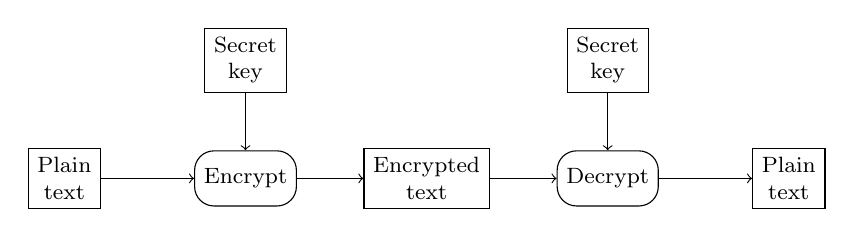
\begin{tikzpicture}[b/.style={draw, font=\footnotesize, align=center, minimum height=0.7cm}, o/.style={draw, rounded corners=7pt, font=\footnotesize, minimum height=0.7cm}]
\node[b] (p1) at (0,0) {Plain\\text};
\node[o] (e) at (2.3,0) {Encrypt};
\node[b] (c) at (4.6,0) {Encrypted\\text};
\node[o] (d) at (6.9,0) {Decrypt};
\node[b] (p2) at (9.2,0) {Plain\\text};
\node[b] (k1) at (2.3,1.5) {Secret\\key};
\node[b] (k2) at (6.9,1.5) {Secret\\key};
\draw[->] (p1) -- (e); \draw[->] (e) -- (c); \draw[->] (c) -- (d); \draw[->] (d) -- (p2);
\draw[->] (k1) -- (e); \draw[->] (k2) -- (d);
\end{tikzpicture}
\caption{Cifratura e decifratura. Il testo in chiaro diventa testo cifrato con una chiave; con una chiave lo si
riporta in chiaro.}
\label{fig:sic-cifratura}
\end{figure}

Le tecniche di cifratura moderne sono considerate ``praticamente inviolabili'' con la tecnologia disponibile oggi. La
storia però insegna che una cifratura apparentemente inviolabile può diventare violabile quando arriva una nuova
tecnologia. Che cosa succederà se un giorno i computer quantistici saranno disponibili in commercio?

\subsection{Cifratura simmetrica e asimmetrica}

Nella \termine{cifratura simmetrica}, usata da secoli, la stessa chiave serve per cifrare e per decifrare
(\figrif{fig:sic-simmetrica}, a sinistra). Il punto debole è \textbf{come condividere la chiave in modo sicuro}:
mittente e destinatario devono averla entrambi, e chi la intercetta legge tutto.

Nella \termine{cifratura asimmetrica} si usano chiavi diverse per cifrare e per decifrare: una \emph{chiave pubblica},
che si può dare a tutti, e una \emph{chiave privata}, che resta al proprietario. Ciò che si cifra con una delle due si
decifra solo con l'altra. La cifratura asimmetrica si usa in due modi (\figrif{fig:sic-simmetrica}, a destra).
\begin{itemize}
  \item \textbf{Riservatezza.} Alice cifra il messaggio con la chiave \emph{pubblica} di Bob. Solo Bob, con la sua
    chiave privata, può decifrarlo.
  \item \textbf{Autenticità.} Bob cifra il messaggio ``I am really Bob'' con la propria chiave \emph{privata}. Alice lo
    decifra con la chiave pubblica di Bob. Se ci riesce, il messaggio può averlo cifrato solo Bob.
\end{itemize}

\begin{figure}[ht]
\centering
\begin{tikzpicture}[b/.style={draw, font=\scriptsize, align=center, minimum height=0.55cm, inner sep=2pt}, k/.style={font=\scriptsize\ttfamily, draw, fill=grigiochiaro, inner sep=2pt}]
% simmetrica
\node[font=\footnotesize\bfseries] at (1.6,2.3) {Simmetrica};
\node[font=\scriptsize] at (0.2,1.85) {Alice};
\node[font=\scriptsize] at (3.0,1.85) {Bob};
\node[k] (ka) at (0.2,1.35) {a7Dr6yYt9F...};
\node[k] (kb) at (3.0,1.35) {a7Dr6yYt9F...};
\node[b] (m1) at (-0.4,0) {Secret\\message};
\node[b] (c1) at (1.6,0) {Encrypted\\text};
\node[b] (m2) at (3.6,0) {Secret\\message};
\draw[->, thick] (m1) -- (c1); \draw[->, thick] (c1) -- (m2);
\draw[->] (ka) -- node[left, font=\scriptsize] {encrypt} (0.6,0.3);
\draw[->] (kb) -- node[right, font=\scriptsize] {decrypt} (2.6,0.3);
% asimmetrica: riservatezza
\node[font=\footnotesize\bfseries] at (7.8,2.3) {Asimmetrica};
\node[font=\scriptsize, align=center] at (6.3,1.85) {chiave pubblica di Bob};
\node[font=\scriptsize, align=center] at (9.3,1.85) {chiave privata di Bob};
\node[k] (pb) at (6.3,1.35) {dr5ts3TR9dt...};
\node[k] (sb) at (9.3,1.35) {hTr34BbfsDy...};
\node[b] (m3) at (5.8,0) {Secret\\message};
\node[b] (c3) at (7.8,0) {Encrypted\\text};
\node[b] (m4) at (9.8,0) {Secret\\message};
\draw[->, thick] (m3) -- (c3); \draw[->, thick] (c3) -- (m4);
\draw[->] (pb) -- node[left, font=\scriptsize] {encrypt} (6.8,0.3);
\draw[->] (sb) -- node[right, font=\scriptsize] {decrypt} (8.8,0.3);
\node[font=\scriptsize, anchor=north] at (7.8,-0.45) {riservatezza: solo Bob legge};
% asimmetrica: autenticita
\node[k] (sb2) at (6.3,-1.85) {hTr34BbfsDy...};
\node[k] (pb2) at (9.3,-1.85) {dr5ts3TR9dt...};
\node[font=\scriptsize] at (6.3,-1.4) {chiave privata di Bob};
\node[font=\scriptsize] at (9.3,-1.4) {chiave pubblica di Bob};
\node[b] (m5) at (5.8,-3.2) {I am\\really Bob};
\node[b] (c5) at (7.8,-3.2) {Encrypted\\text};
\node[b] (m6) at (9.8,-3.2) {I am\\really Bob};
\draw[->, thick] (m5) -- (c5); \draw[->, thick] (c5) -- (m6);
\draw[->] (sb2) -- node[left, font=\scriptsize] {encrypt} (6.8,-2.9);
\draw[->] (pb2) -- node[right, font=\scriptsize] {decrypt} (8.8,-2.9);
\node[font=\scriptsize, anchor=north] at (7.8,-3.65) {autenticità: solo Bob può averlo scritto};
\end{tikzpicture}
\caption{Cifratura simmetrica e asimmetrica. A sinistra Alice e Bob usano la stessa chiave. A destra, in alto, si cifra
con la chiave pubblica di Bob e solo la sua chiave privata decifra; in basso Bob cifra con la propria chiave privata e
chiunque, con la chiave pubblica, verifica che il messaggio viene da lui.}
\label{fig:sic-simmetrica}
\end{figure}

\subsection{TLS e certificati digitali}
\label{sec:sic-tls}

\begin{itemize}
  \item HTTPS è HTTP più \termine{TLS} (\ingl{Transport Layer Security}, che ha sostituito SSL).
  \item TLS serve a verificare l'identità del web server e a cifrare le comunicazioni.
  \item La cifratura TLS usa un \termine{certificato digitale} che il server manda al client.
  \item I certificati digitali sono emessi da un servizio di fiducia che verifica le identità, la \termine{certificate
    authority} (CA).
\end{itemize}

Client e server interagiscono per generare una \textbf{chiave simmetrica} con cui scambiarsi i dati. Così sfruttano
la cifratura asimmetrica per mettersi d'accordo e quella simmetrica, più veloce, per i dati
(\figrif{fig:sic-tls}).

\begin{algoritmo}[Handshake TLS]
\begin{enumerate}
  \item Il client manda un \emph{Hello} con i metodi di cifratura che supporta.
  \item Il server risponde con un \emph{Hello} che indica il metodo da usare.
  \item Il client chiede al server di provare la propria identità.
  \item Il server genera un grande numero casuale RS, lo cifra con la propria chiave privata e manda al client il
    certificato digitale insieme a RS cifrato.
  \item Il client controlla l'emittente del certificato, la sua validità e la firma digitale. Genera un grande numero
    casuale RC. Decifra RS e cifra RC con la chiave pubblica presa dal certificato, poi manda RC cifrato al server.
  \item Il server decifra RC con la propria chiave privata.
  \item Client e server calcolano entrambi la chiave simmetrica a partire da RS e RC.
  \item Si scambiano i dati cifrati con la chiave simmetrica, fino alla fine della sessione.
\end{enumerate}
\end{algoritmo}

\begin{figure}[ht]
\centering
\begin{tikzpicture}[s/.style={draw, fill=white, font=\scriptsize, minimum width=1.4cm, align=center, inner sep=2pt}]
\node[font=\footnotesize\bfseries] at (0,0.45) {Client};
\node[font=\footnotesize\bfseries] at (6,0.45) {Server};
\draw[very thick, blu] (0,0.2) -- (0,-9.6);
\draw[very thick, blu] (6,0.2) -- (6,-9.6);
\node[s] at (0,-0.2) {Hello};
\draw[->] (0.7,-0.2) -- node[above, font=\scriptsize] {Encryption methods supported} (6,-0.2);
\node[s] at (6,-0.9) {Hello};
\draw[->] (5.3,-0.9) -- node[above, font=\scriptsize] {Encryption method to be used} (0,-0.9);
\node[s] at (0,-1.6) {Verify};
\draw[->] (0.7,-1.6) -- node[above, font=\scriptsize] {Prove your identity} (6,-1.6);
\node[s] at (6,-2.3) {Generate RS};
\node[font=\scriptsize, anchor=west] at (6.8,-2.3) {RS: grande numero casuale};
\node[s] at (6,-3.0) {Encrypt RS};
\node[font=\scriptsize, anchor=west] at (6.8,-3.0) {con la chiave privata};
\node[s] at (6,-3.7) {Get certificate};
\draw[->] (5.3,-3.95) -- node[above, font=\scriptsize] {Digital certificate + encrypted RS} (0,-3.95);
\node[s] at (0,-4.6) {Check\\certificate};
\node[font=\scriptsize, anchor=east, align=right] at (-0.8,-4.6) {emittente, validità e\\firma del certificato};
\node[s] at (0,-5.4) {Generate RC};
\node[font=\scriptsize, anchor=east] at (-0.8,-5.4) {RC: grande numero casuale};
\node[s] at (0,-6.1) {Decrypt RS\\Encrypt RC};
\node[font=\scriptsize, anchor=east, align=right] at (-0.8,-6.1) {con la chiave pubblica\\del certificato};
\draw[->] (0.7,-6.6) -- node[above, font=\scriptsize] {Encrypted RC} (6,-6.6);
\node[s] at (6,-7.1) {Decrypt RC};
\node[font=\scriptsize, anchor=west] at (6.8,-7.1) {con la chiave privata};
\node[s] at (0,-7.8) {Compute key};
\node[s] at (6,-7.8) {Compute key};
\node[font=\scriptsize, anchor=west] at (6.8,-7.8) {chiave simmetrica da RS e RC};
\node[s] at (0,-8.6) {Exchange data};
\node[s] at (6,-8.6) {Exchange data};
\draw[<->] (1.0,-8.6) -- node[above, font=\scriptsize] {dati cifrati} (5.0,-8.6);
\node[s] at (0,-9.3) {End session};
\node[s] at (6,-9.3) {End session};
\end{tikzpicture}
\caption{Handshake TLS. Il tempo scorre verso il basso. Il server prova la propria identità con il certificato;
client e server si scambiano due numeri casuali, RS e RC, e ne ricavano la stessa chiave simmetrica, usata per
cifrare i dati della sessione.}
\label{fig:sic-tls}
\end{figure}

\subsection{Cifrare i dati}
\label{sec:sic-dati}

I dati degli utenti vanno cifrati ogni volta che è possibile.
\begin{itemize}
  \item I dati \textbf{in transito} vanno sempre cifrati.
  \item I dati \textbf{a riposo} (\ingl{at rest}), cioè memorizzati, vanno sempre cifrati.
  \item Cifrare e decifrare i dati \textbf{in uso}, cioè mentre sono elaborati, rallenta il tempo di risposta del sistema.
\end{itemize}
La cifratura dei dati è possibile a quattro livelli del sistema (\tabrif{tab:sic-livelli}).

\begin{table}[ht]
\centering
\small
\caption{I quattro livelli a cui si possono cifrare i dati.}
\label{tab:sic-livelli}
\begin{tabularx}{\linewidth}{>{\raggedright\arraybackslash}p{2.0cm}X>{\raggedright\arraybackslash}p{3.3cm}}
\toprule
Livello & Che cosa si cifra & Note \\
\midrule
Application & L'applicazione decide quali dati cifrare; li decifra subito prima di usarli. & problemi di prestazioni;
  serve la gestione delle chiavi \\
Database & Il DBMS può cifrare l'intero database quando è chiuso e decifrarlo quando è riaperto. In alternativa può
  cifrare e decifrare singole tabelle o colonne. & \\
Files & Il sistema operativo cifra i singoli file quando sono chiusi e li decifra quando sono riaperti. & \\
Media & Il sistema operativo cifra i dischi quando sono smontati e li decifra quando sono rimontati. & utile per
  portatili rubati o persi \\
\bottomrule
\end{tabularx}
\end{table}

\subsection{Gestione delle chiavi}
\label{sec:sic-chiavi}

\begin{attenzione}[Chiavi perse, dati persi]
\uline{Se le chiavi vanno perse, i dati cifrati diventano inaccessibili per sempre.}
\end{attenzione}

\begin{itemize}
  \item Le norme sulla protezione dei dati possono imporre di conservare copie dei dati per anni, in modo sicuro.
  \item Le chiavi vanno cambiate periodicamente. Bisogna quindi conservare più versioni delle chiavi, ciascuna con la
    propria data.
  \item Si usa un \termine{key management system} (KMS) per garantire che le chiavi siano generate, conservate e
    consultate in modo sicuro, e solo dagli utenti autorizzati (\figrif{fig:sic-kms}).
\end{itemize}

\begin{figure}[ht]
\centering
\begin{tikzpicture}[b/.style={draw, rounded corners=6pt, font=\footnotesize, align=center, minimum width=2.3cm, minimum height=0.7cm}, r/.style={draw, font=\footnotesize, align=center, minimum width=2.3cm, minimum height=0.7cm}]
\node[b] (app) at (3.0,2.4) {Application};
\node[r] (api) at (0,1.0) {API};
\node[b, anchor=north] (kms) at (api.south) {Key management\\system};
\node[r] (ks) at (0,-1.6) {Key store};
\node[r] (ud) at (6.0,1.0) {Unencrypted data};
\node[b] (ee) at (6.0,-0.2) {Encryption\\engine};
\node[r] (sd) at (6.0,-1.6) {Stored encrypted\\data};
\draw[->, very thick, blu] (app.west) -| node[pos=0.75, right, font=\scriptsize] {Calls} (api.north);
\draw[<->, very thick, blu] (app.east) -| (ud.north);
\draw[<->, very thick, blu] (ud) -- (ee);
\draw[<->, very thick, blu] (ee) -- (sd);
\draw[<->, very thick, blu] (kms) -- (ks);
\draw[->, very thick, blu] (kms.east) -- node[below, font=\scriptsize] {Keys} (ee.west);
\end{tikzpicture}
\caption{Key management system. L'applicazione chiede le chiavi al KMS attraverso la sua API. Il KMS le conserva nel
key store e le passa al motore di cifratura, che trasforma i dati in chiaro dell'applicazione nei dati cifrati
memorizzati, e viceversa.}
\label{fig:sic-kms}
\end{figure}

\section{Privacy}
\label{sec:sic-privacy}

\begin{definizione}[Privacy]
La \termine{privacy} è un concetto sociale che riguarda la raccolta, la diffusione e l'uso appropriato delle
informazioni personali conservate da una terza parte.
\end{definizione}

Le leggi sulla protezione dei dati definiscono le responsabilità di chi tratta i dati e i diritti delle persone a cui i
dati si riferiscono (\figrif{fig:sic-leggi}). Il \termine{data controller} è chi decide come e perché trattare i dati
personali; il \termine{data subject} è la persona a cui i dati si riferiscono.

\begin{figure}[ht]
\centering
\begin{tikzpicture}[e/.style={draw, ellipse, font=\footnotesize, align=center, inner sep=2pt}]
\node[e] (l) at (0,0) {Data protection\\laws};
\node[e] (c) at (-4.0,1.0) {Responsibilities of\\the data controller};
\node[e] (s) at (4.0,1.0) {Rights of the\\data subject};
\draw (l) -- (c); \draw (l) -- (s);
\node[font=\footnotesize, align=center, anchor=north] at (-4.0,0.3) {Data storage\\Data use\\Security\\Subject access};
\node[font=\footnotesize, align=center, anchor=north] at (4.0,0.3) {Data access\\Error correction\\Data deletion\\Consent};
\end{tikzpicture}
\caption{Le leggi sulla protezione dei dati. Il data controller è responsabile di memorizzazione, uso e sicurezza dei
dati e dell'accesso degli interessati. Il data subject ha diritto di accedere ai propri dati, di correggerli, di
cancellarli e di dare o negare il consenso.}
\label{fig:sic-leggi}
\end{figure}

\begin{table}[ht]
\centering
\small
\caption{Principi di protezione dei dati.}
\label{tab:sic-principi}
\begin{tabularx}{\linewidth}{>{\raggedright\arraybackslash}p{3.6cm}X}
\toprule
Principio & Spiegazione \\
\midrule
Awareness and control & Gli utenti devono sapere quali dati si raccolgono quando usano il prodotto, e devono avere
  il controllo delle informazioni personali raccolte su di loro. \\
Purpose & Bisogna dire agli utenti perché si raccolgono i dati, e non usarli per altri scopi. \\
Consent & Serve sempre il consenso dell'utente prima di comunicare i suoi dati ad altri. \\
Data lifetime & Non si conservano i dati più del necessario. Se un utente cancella l'account, si cancellano i dati
  personali associati. \\
Secure storage & I dati si conservano in modo sicuro, perché non possano essere manomessi o rivelati a persone non
  autorizzate. \\
Discovery and error correction & Gli utenti devono poter scoprire quali dati personali si conservano su di loro, e
  devono avere un modo per correggerne gli errori. \\
Location & Non si conservano dati in paesi con leggi sulla protezione dei dati più deboli, a meno di un accordo
  esplicito che faccia valere le regole più forti. \\
\bottomrule
\end{tabularx}
\end{table}

\tabrif{tab:sic-principi} riassume i principi di protezione dei dati. Ci sono anche ragioni di business per curare la
privacy delle informazioni.
\begin{itemize}
  \item Se il prodotto non rispetta le norme sulla protezione dei dati, si rischiano azioni legali, oppure non si può
    vendere il prodotto.
  \item Chi vende un prodotto aziendale può ricevere dai clienti la richiesta di garanzie sulla privacy: i clienti non
    vogliono essere a rischio con i propri utenti.
  \item La fuga o l'uso improprio delle informazioni dei clienti può danneggiare la reputazione.
\end{itemize}

Le informazioni che il software deve raccogliere dipendono dalle funzionalità del prodotto e dal modello di business.
Alcuni consigli:
\begin{itemize}
  \item non raccogliere informazioni personali che non servono;
  \item stabilire una \emph{privacy policy} che definisca come si raccolgono, si conservano e si gestiscono le
    informazioni personali e sensibili degli utenti;
  \item dire chiaramente se si usano i dati degli utenti per la pubblicità mirata o per offrire servizi pagati da
    altre aziende;
  \item se il prodotto ha funzioni di social network con cui gli utenti condividono informazioni, assicurarsi che gli
    utenti capiscano come controllare ciò che condividono.
\end{itemize}

\begin{puntichiave}
\begin{itemize}
  \item Minacce alla disponibilità, all'integrità e alla riservatezza. La sicurezza riguarda tutto lo stack, dalla
    rete all'applicazione.
  \item Attacchi e difese:
    \begin{itemize}
      \item injection (buffer overflow, SQL poisoning): validare l'input;
      \item session hijacking: HTTPS, più fattori, timeout brevi;
      \item cross-site scripting: validare e codificare;
      \item DoS e DDoS: filtri, blocchi temporanei, tracciamento IP;
      \item brute force: password lunghe, due fattori.
    \end{itemize}
  \item Autenticazione: knowledge-, possession-, attribute-based, spesso a più fattori. L'identità federata (OAuth)
    affida l'autenticazione a un servizio di fiducia.
  \item Autenticazione $\neq$ autorizzazione. L'autorizzazione si realizza con le ACL, organizzate per gruppi.
  \item Cifratura simmetrica (una chiave condivisa) e asimmetrica (chiave pubblica e privata). TLS usa l'asimmetrica e
    i certificati per concordare una chiave simmetrica.
  \item Dati sempre cifrati in transito e a riposo; quattro livelli di cifratura; senza chiavi i dati sono persi: KMS.
  \item Privacy: principi di protezione dei dati, ragioni di business, raccogliere solo i dati necessari.
\end{itemize}
\end{puntichiave}

\begin{domande}
\begin{enumerate}
  \item Quali sono i tre tipi di minacce? Fare un esempio di attacco che ne combina due.
  \item Perché la sicurezza riguarda tutto il sistema? Quali attività di gestione la mantengono?
  \item Come funziona un attacco di SQL poisoning? Come ci si difende?
  \item Che cos'è il session hijacking? Come si ottiene il cookie di sessione? Quali difese ci sono?
  \item Descrivere un attacco di cross-site scripting e le sue difese.
  \item Che cosa sono DoS e DDoS? Come può un attacco DoS colpire un singolo utente?
  \item Quali sono gli approcci all'autenticazione? Quali sono le debolezze delle password?
  \item Quali sono vantaggi e svantaggi dell'identità federata?
  \item Che differenza c'è tra autenticazione e autorizzazione? Che cosa sono le ACL?
  \item Confrontare cifratura simmetrica e asimmetrica. Come si usa la cifratura asimmetrica per l'autenticità?
  \item Descrivere l'handshake TLS.
  \item A quali livelli si possono cifrare i dati? Perché serve un key management system?
  \item Quali sono i principi di protezione dei dati?
\end{enumerate}
\end{domande}
